\documentclass{article}
\usepackage[margin=1in]{geometry}
\usepackage{graphicx}
\usepackage{xcolor}
\usepackage{float}
\usepackage{amsmath}
\usepackage{cite}
\usepackage{hyperref}
\usepackage{indentfirst}
\graphicspath{{..} {./images}}

\definecolor{navy-blue}{rgb}{0.22,0.38,0.71}

\renewcommand{\contentsname}{\vspace*{-2\baselineskip}}

\hypersetup{
	colorlinks,
	linkcolor=black,
	urlcolor=blue,
	citecolor=black
}
  		
\begin{document}
\begin{titlepage}
	\centering
	{\huge Lab 7 - Digital Modulation: Frame Synchronization}\\[0.25 in]
	
\includegraphics[width=0.6\textwidth]{ua_logo.png}\\[0.25 in]
	{\large \textbf{ECE 531 - Software Defined Radio\\[0.25 in]
	April 18, 2025\\[0.25 in]}}
	{\large Owen Sowatzke, osowatzke@arizona.edu\\[0.05 in]
	Department of Electrical \& Computer Engineering\\[0.05 in]
	University of Arizona, Tucson, AZ 85721\\[0.5 in]}
	\hypersetup{linkcolor=navy-blue}
	\noindent\hrulefill
	\tableofcontents
	\noindent\hrulefill
\end{titlepage}

% \setlength{\parindent}{0pt}

\section{Introduction}
%Introduction to the laboratory experiment, including a brief description of the objectives and goals.

In this lab, we perform frame synchronization on data generated in MATLAB. Correct frame alignment is critical for correctly recovering the transmitted data. To detect the start of a packet, we specifically cross-correlate our received data with a known preamble. As part of our work in this lab, we learn how to perform cross-correlation with MATLAB's \texttt{filter} command. We also explore perform tradeoffs between the \texttt{xcorr} and \texttt{filter} commands. Finally, we implement a custom frame synchronization routine and evaluate its detection probabilities and packet error rates. The work that follows is divided into two sections. One provides the procedures for each of our experiments, and the other presents the results.

\section{Procedure}
% Detailed explanation of the laboratory experiment, including the design, implementation, and testing of the system.

\section{Results}
% Results and discussion of the laboratory experiment, including captured outputs, observations, and responses to laboratory questions.

\begin{figure}[H]
	\centerline{\fbox{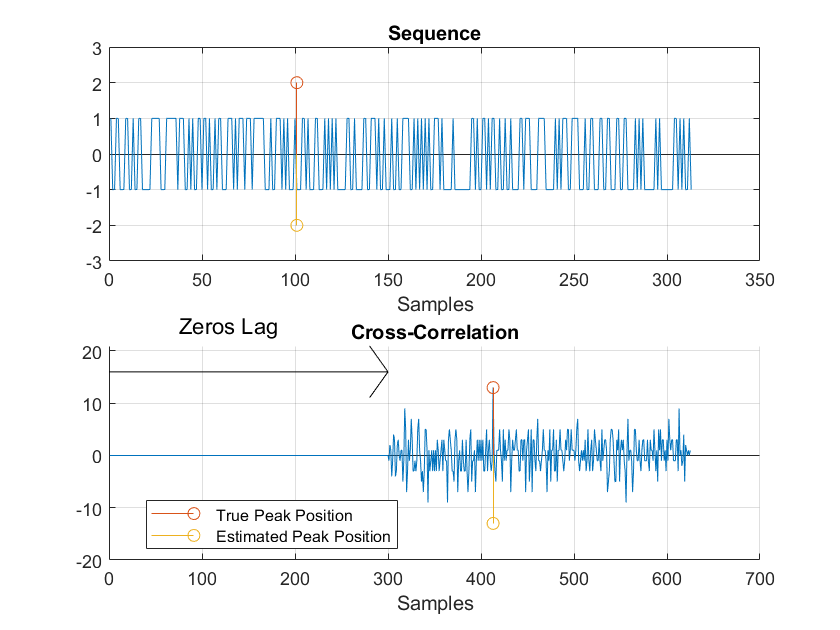
\includegraphics[width=0.5\textwidth]{xcorr_preamble_detect.png}}}
	\caption{Detecting Start of Preamble with \texttt{xcorr} Command}
	\label{fig::xcorr_preamble_detect}
\end{figure}

\begin{figure}[H]
	\centerline{\fbox{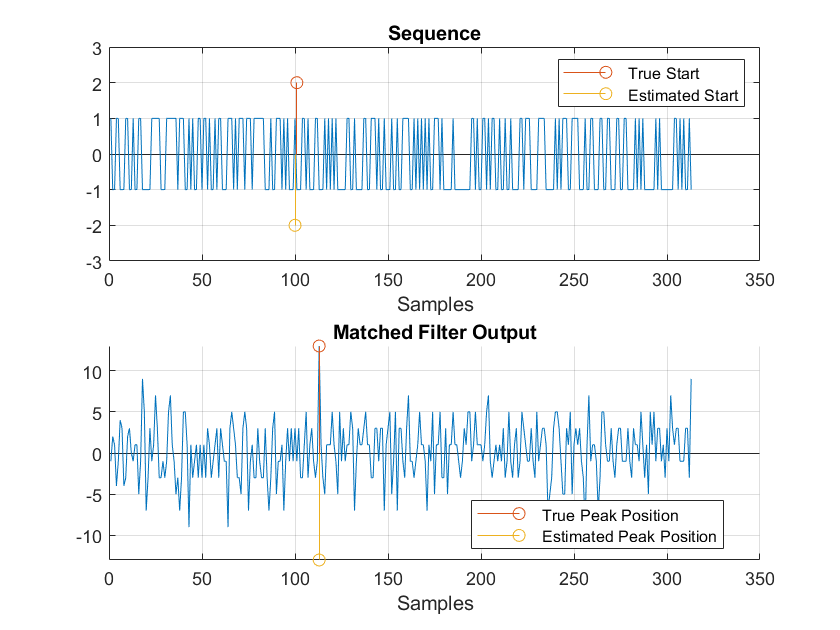
\includegraphics[width=0.5\textwidth]{filter_preamble_detect.png}}}
	\caption{Detecting Start of Preamble with \texttt{filter} Command}
	\label{fig::filter_preamble_detect}
\end{figure}

\begin{figure}[H]
	\centerline{\fbox{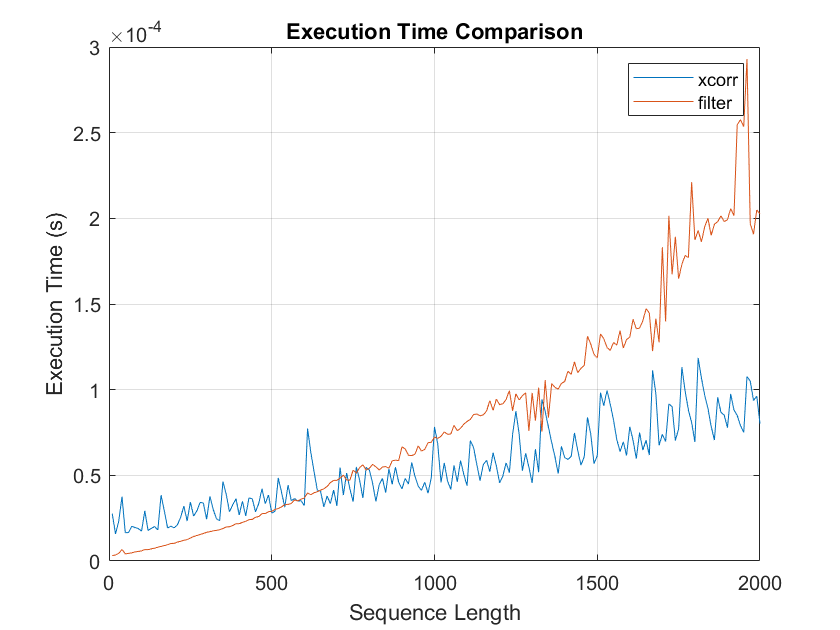
\includegraphics[width=0.5\textwidth]{execution_time.png}}}
	\caption{Comparison of \texttt{filter} and \texttt{filter} Execution Time}
	\label{fig::execution_time}
\end{figure}

\begin{figure}[H]
	\centerline{\fbox{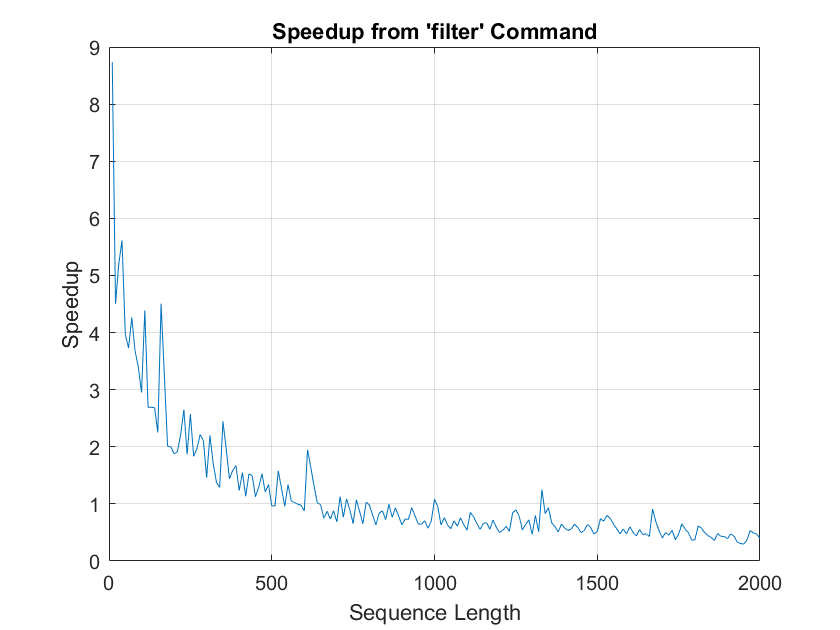
\includegraphics[width=0.5\textwidth]{speedup.png}}}
	\caption{Speedup from \texttt{filter} Command}
	\label{fig::speedup}
\end{figure}

\section{Conclusion}
% Conclusions to the overall lab that discuss meaningful lessons learned and other takeaways from the assignment. (Important)

\end{document}